Im folgenden Abschnitt sind die während des Versuches aufgenommenen Messwerte und die 
aus diesen berechneten Ergebnisse tabellarisch aufgeführt. An entsprechender Stelle
sind Erklärungen und Anmerkungen zu den angestellten Rechnungen und Ergebnissen gegeben.
Die Fehler der Messwerte wurden allgemein mit der kleinsten Skaleneinteilung des jeweiligen 
Messgerätes abgeschätzt.
%Die für die Fehlerrechnung verwendeten Fehlergleichungen befinden sich im \cref{sec:Fehlerrechnung}
%und werden mit römischen Ziffern referenziert.


\subsection{Messung des Photostroms für die Spektrallinien von Quecksilber}

		
		Die Messwerte für die fünf untersuchten Spektrallinie des Quecksilbers sind
		in den Tabellen \ref{tab:Messwerte_Orange} bis \ref{tab:Messwerte_Violett2} aufgeführt.
		
		\begin{table}[!h]
	\centering
	\begin{tabular}{|c|c||c|c|}
		\hline
		Photostrom & Bremsspannung & Photostrom & Bremsspannung\\
		$I$ [\si{\pico\ampere}] & $U$ [\si{\volt}] & $I$ [\si{\pico\ampere}] & $U$ [\si{\volt}]\\
\hline\hline
		\num{0.0(5)} & \num{0.368(1)} & \num{5.0(5)} & \num{0.139(1)}\\
		\num{1.0(5)} & \num{0.293(1)} & \num{6.0(5)} & \num{0.114(1)}\\
		\num{2.0(5)} & \num{0.250(1)} & \num{7.0(5)} & \num{0.101(1)}\\
		\num{3.0(5)} & \num{0.183(1)} & \num{8.0(5)} & \num{0.076(1)}\\
		\num{4.0(5)} & \num{0.157(1)} & \num{9.0(5)} & \num{0.065(1)}\\
		\hline
	\end{tabular}
	\caption{Messwerte der orangenen Spektrallinie \label{tab:Messwerte_Orange}}
\end{table}

		\begin{table}[!h]
	\centering
	\begin{tabular}{|c|c|c|c|}
		\hline
		Photostrom & Bremsspannung & Photostrom & Bremsspannung\\
		$I$ [\si{\pico\ampere}] & $U$ [\si{\volt}] & $I$ [\si{\pico\ampere}] & $U$ [\si{\volt}]\\
\hline\hline
		\num{0.0(5)} & \num{0.398(1)} & \num{16.0(5)} & \num{0.206(1)}\\
		\num{2.0(5)} & \num{0.348(1)} & \num{18.0(5)} & \num{0.194(1)}\\
		\num{4.0(5)} & \num{0.318(1)} & \num{20.0(5)} & \num{0.182(1)}\\
		\num{6.0(5)} & \num{0.293(1)} & \num{30.0(5)} & \num{0.126(1)}\\
		\num{8.0(5)} & \num{0.268(1)} & \num{40.0(5)} & \num{0.095(1)}\\
		\num{10.0(5)} & \num{0.250(1)} & \num{50.0(5)} & \num{0.057(1)}\\
		\num{12.0(5)} & \num{0.237(1)} & \num{60.0(5)} & \num{0.027(1)}\\
		\num{14.0(5)} & \num{0.219(1)} & \num{70.0(5)} & \num{0.000(1)}\\
		\hline
	\end{tabular}
	\caption{Messwerte der grünen Spektrallinie \label{tab:Messwerte_Gruen}}
\end{table}

		\begin{table}[!h]
	\centering
	\begin{tabular}{|c|c||c|c|}
		\hline
		Photostrom & Bremsspannung & Photostrom & Bremsspannung\\
		$I$ [\si{\pico\ampere}] & $U$ [\si{\volt}] & $I$ [\si{\pico\ampere}] & $U$ [\si{\volt}]\\
\hline\hline
		\num{0.0(5)} & \num{0.460(1)} & \num{3.0(5)} & \num{0.200(1)}\\
		\num{1.0(5)} & \num{0.411(1)} & \num{4.0(5)} & \num{0.157(1)}\\
		\num{1.5(5)} & \num{0.355(1)} & \num{4.5(5)} & \num{0.100(1)}\\
		\num{2.0(5)} & \num{0.300(1)} & \num{5.0(5)} & \num{0.070(1)}\\
		\num{2.5(5)} & \num{0.250(1)} & \num{6.0(5)} & \num{0.000(1)}\\
		\hline
	\end{tabular}
	\caption{Messwerte der cyanen Spektrallinie \label{tab:Messwerte_Cyan}}
\end{table}

		\begin{table}[!h]
	\centering
	\begin{tabular}{|c|c|c|c|}
		\hline
		Photostrom & Bremsspannung & Photostrom & Bremsspannung\\
		$I$ [\si{\pico\ampere}] & $U$ [\si{\volt}] & $I$ [\si{\pico\ampere}] & $U$ [\si{\volt}]\\
\hline\hline
		\num{0.0(5)} & \num{0.825(1)} & \num{112.0(5)} & \num{0.367(1)}\\
		\num{10.0(5)} & \num{0.752(1)} & \num{160.0(5)} & \num{0.259(1)}\\
		\num{24.0(5)} & \num{0.677(1)} & \num{185.0(5)} & \num{0.206(1)}\\
		\num{44.0(5)} & \num{0.590(1)} & \num{245.0(5)} & \num{0.101(1)}\\
		\num{84.0(5)} & \num{0.455(1)} & \num{300.0(5)} & \num{0.000(1)}\\
		\hline
	\end{tabular}
	\caption{Messwerte der ersten violetten Spektrallinie \label{tab:Messwerte_Violett1}}
\end{table}

		\begin{table}[!h]
	\centering
	\begin{tabular}{|c|c||c|c|}
		\hline
		Photostrom & Bremsspannung & Photostrom & Bremsspannung\\
		$I$ [\si{\pico\ampere}] & $U$ [\si{\volt}] & $I$ [\si{\pico\ampere}] & $U$ [\si{\volt}]\\
\hline\hline
		\num{0.0(5)} & \num{0.943(1)} & \num{34.0(5)} & \num{0.400(1)}\\
		\num{4.0(5)} & \num{0.819(1)} & \num{46.0(5)} & \num{0.306(1)}\\
		\num{10.0(5)} & \num{0.721(1)} & \num{58.0(5)} & \num{0.206(1)}\\
		\num{18.0(5)} & \num{0.615(1)} & \num{70.0(5)} & \num{0.115(1)}\\
		\num{26.0(5)} & \num{0.515(1)} & \num{88.0(5)} & \num{0.000(1)}\\
		\hline
	\end{tabular}
	\caption{Messwerte der zweiten violetten Spektrallinie \label{tab:Messwerte_Violett2}}
\end{table}

		
		In den Abbildungen \ref{fig:Messwerte_Orange} bis \ref{fig:Messwerte_Violett2} sind die 
		radizierten Messwerte des Photostroms gegen die Bremsspannung und die 
		mit Hilfe der Python-Bibliothek \emph{SciPy} \cite{SciPy} erstellte Regressiongerade 
		eingetragen. 
		Die Regressionsparameter für den Ansatz
		\begin{empheq}{equation}
			I_{w}(U) = a \cdot U + b
		\end{empheq}
		sind für die fünf Spektrallinien in \cref{tab:Messwerte_ParameterSpektrum} zusammen mit  
		den ebenfalls eingezeichneten Grenzspannungen zu finden.
		
		\begin{table}[!h]
	\centering
	\begin{tabular}{|c|c|c|c|c|}
		\hline
		Wellenlänge & Frequenz & Steigung & y-Achsenabschnitt & Grenzspannung\\
		$\lambda$ [\si{\nano\meter}] & $f$ [\si{\peta\hertz}] & $a$ & $b$ & $U_{g}$ [\si{\volt}]\\
\hline\hline
		\num{578} & \num{0.519} & \num{-9.5(5)} & \num{3.59(5)} & \num{0.379}\\
		\num{546} & \num{0.549} & \num{-20.7(3)} & \num{8.29(4)} & \num{0.401}\\
		\num{492} & \num{0.609} & \num{-3.5(1)} & \num{2.47(2)} & \num{0.705}\\
		\num{436} & \num{0.688} & \num{-18.3(2)} & \num{17.39(5)} & \num{0.949}\\
		\num{405} & \num{0.740} & \num{-8.5(1)} & \num{9.37(4)} & \num{1.097}\\
		\hline
	\end{tabular}
	\caption{Regressionsparameter der Untersuchung der Spektrallinien \label{tab:Messwerte_ParameterSpektrum}}
\end{table}

		
		\begin{figure}[!h]
			\centering
			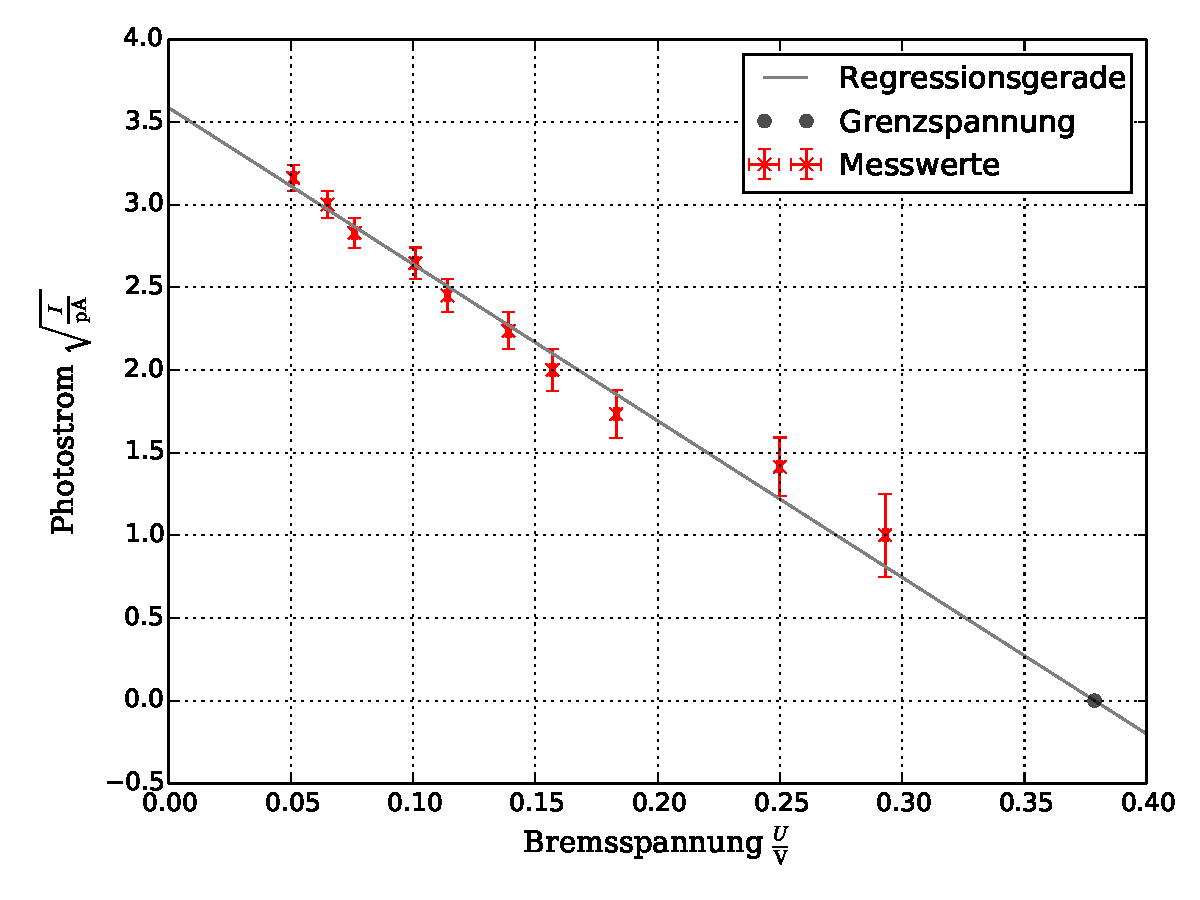
\includegraphics[scale=0.7]{Grafiken/Orange.pdf}
			\caption{Messwerte und Regeression der orangenen Linie \label{fig:Messwerte_Orange}}
		\end{figure}
		\begin{figure}[!h]
			\centering
			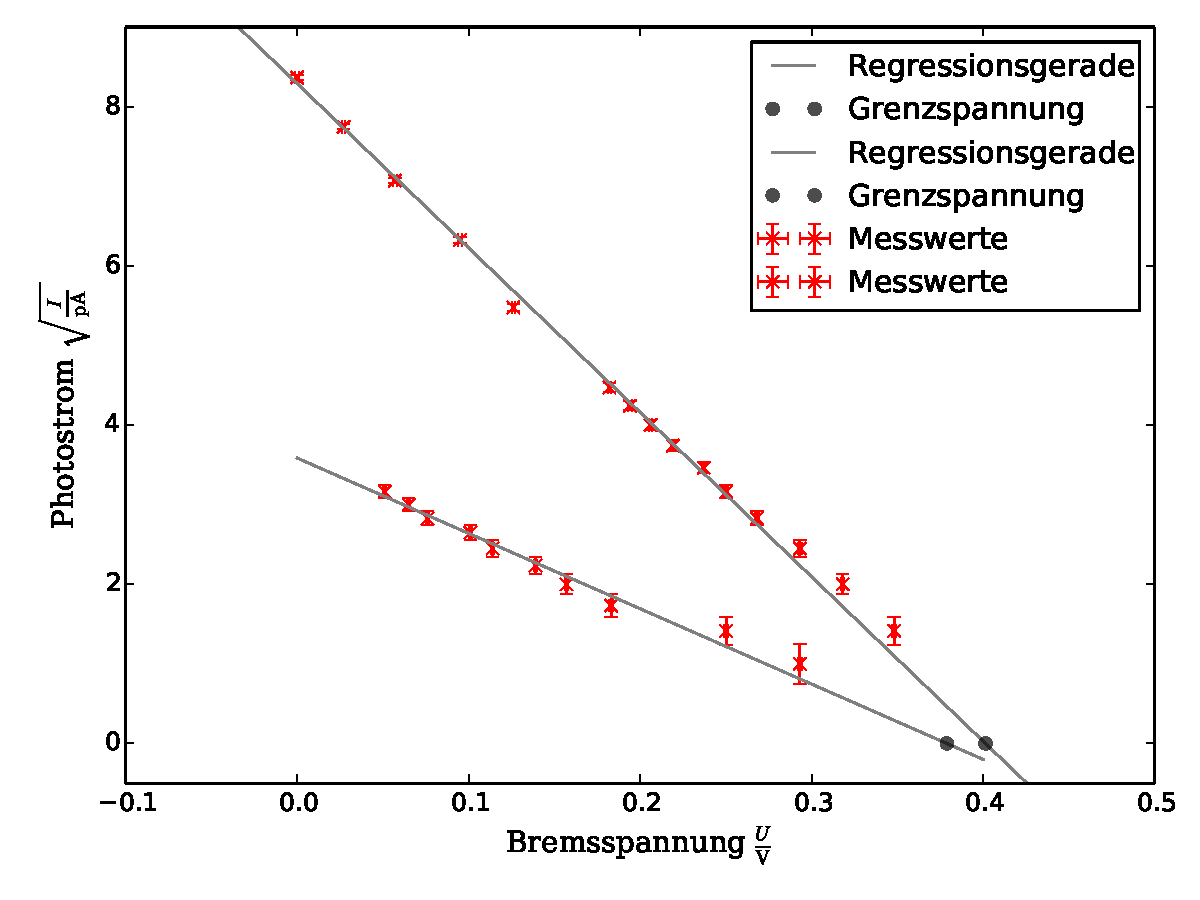
\includegraphics[scale=0.7]{Grafiken/Gruen.pdf}
			\caption{Messwerte und Regeression der grünen Linie \label{fig:Messwerte_Gruen}}
		\end{figure}
		\begin{figure}[!h]
			\centering
			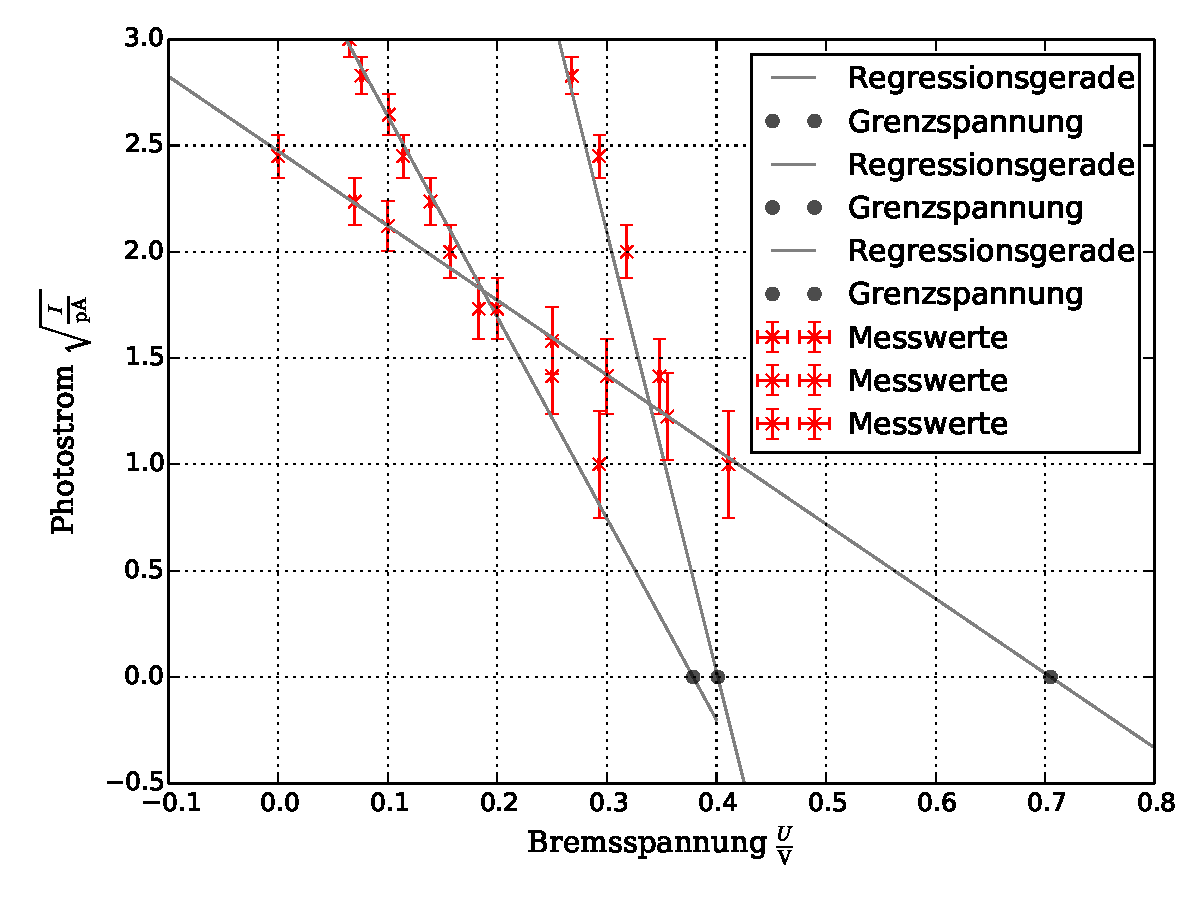
\includegraphics[scale=0.7]{Grafiken/Cyan.pdf}
			\caption{Messwerte und Regeression der cyanen Linie \label{fig:Messwerte_Cyan}}
		\end{figure}
		\begin{figure}[!h]
			\centering
			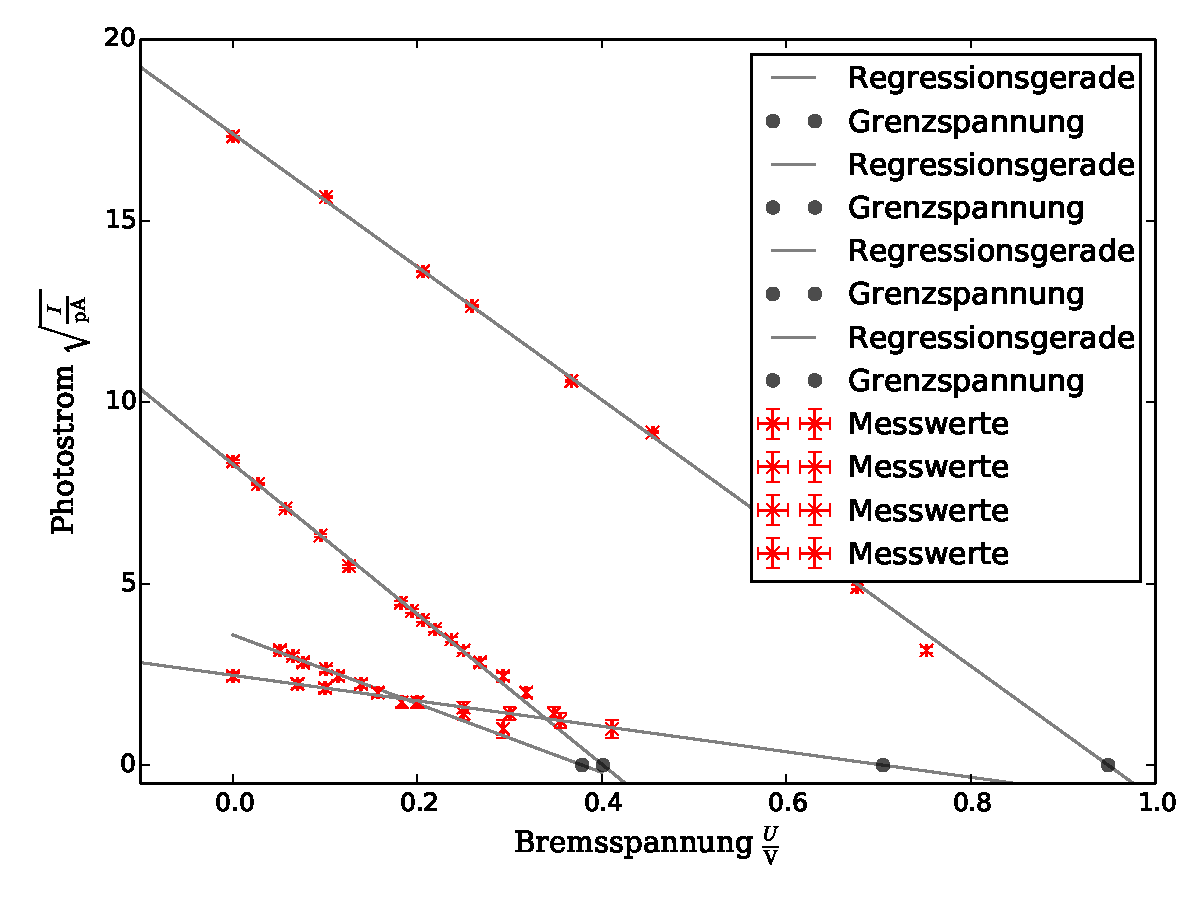
\includegraphics[scale=0.7]{Grafiken/Violett1.pdf}
			\caption{Messwerte und Regeression der ersten violetten Linie \label{fig:Messwerte_Violett1}}
		\end{figure}
		\begin{figure}[!h]
			\centering
			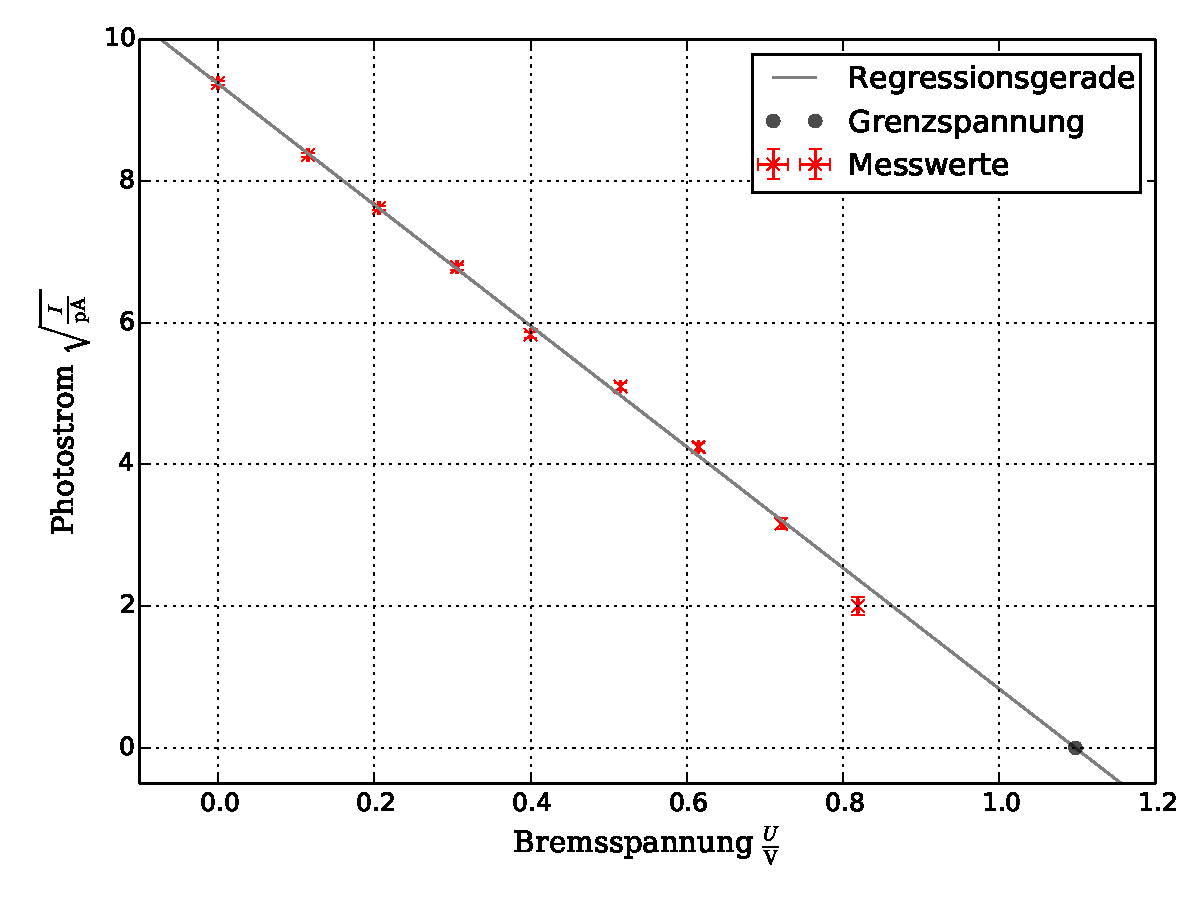
\includegraphics[scale=0.7]{Grafiken/Violett2.pdf}
			\caption{Messwerte und Regeression der zweiten violetten Linie \label{fig:Messwerte_Violett2}}
		\end{figure}
		
		Die berechneten Werte für die Grenzspannungen aus \cref{tab:Messwerte_ParameterSpektrum} 
		sind in \cref{fig:Messwerte_2} gegen die jeweilige Frequenz der Spektrallinie aufgetragen
		und wiederum eine lineare Regression durchgeführt.	
		
		\begin{figure}[!h]
			\centering
			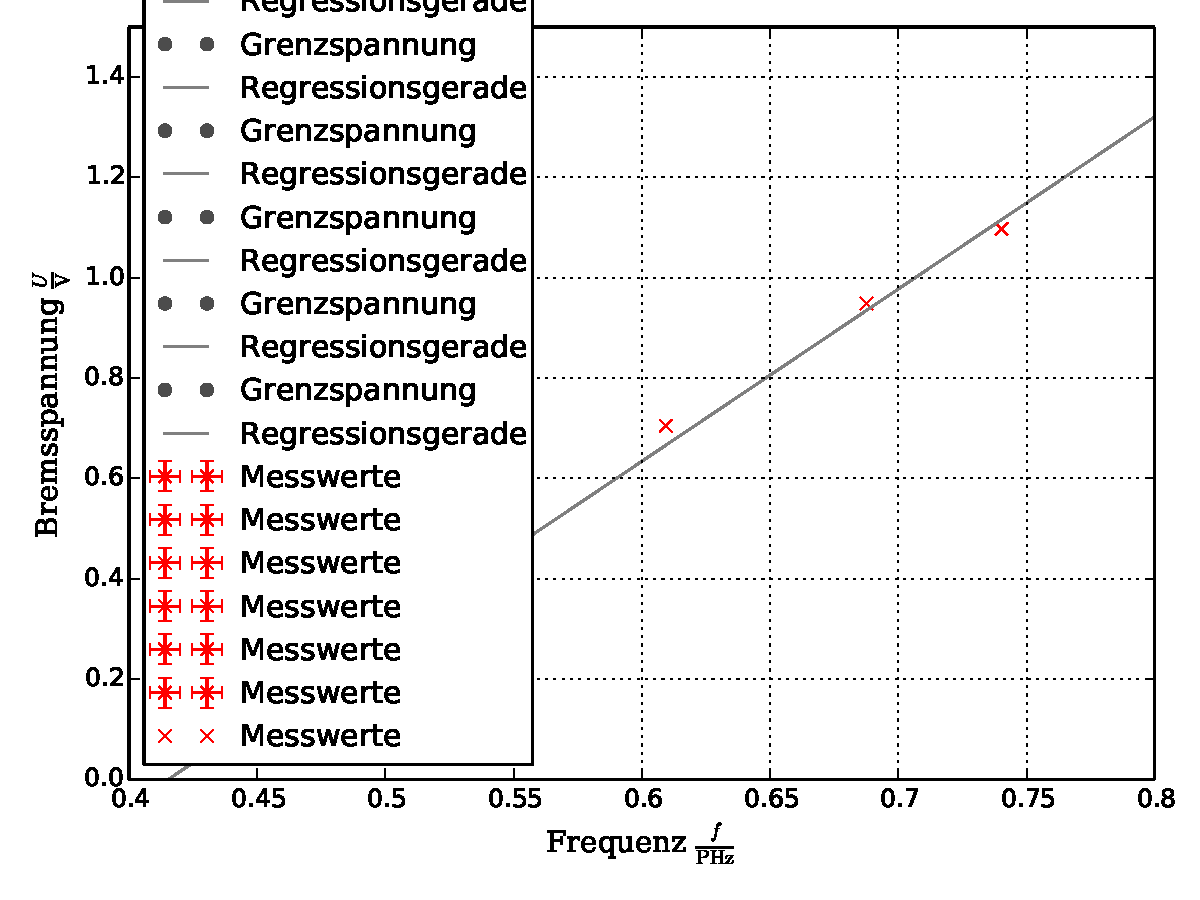
\includegraphics[scale=0.7]{Grafiken/Messreihe2.pdf}
			\caption{Grenzspannung in Abhängigkeit der Frequenz \label{fig:Messwerte_Messwert2}}
		\end{figure}
		
		Die Regression mit dem Ansatz
		\begin{empheq}{equation}
		U_{g}(f) = c \cdot f + d
		\end{empheq}	 
		\addtocounter{equation}{-1}
		\begin{subequations}
			\begin{empheq}{align}
			c &= \SI{3.4(2)e-15}{\volt\second}\\
			d &= \SI{-1.4(2)}{\volt}
			\end{empheq}
		\end{subequations}
		
		Durch Umformung von \cref{eq:} erhält man eine Gerade der Form $U_{g} = \frac{h}{e_{0}}f - \frac{A_{k}}{e_{0}}$. Daraus ergibt sich,
		dass die Steigung der Regressionsgeraden $c$ dem gesuchten Wert für $\tfrac{h}{e_{0}}$ und der Betrag des berechneten
		y-Achsenabschnitts $d$, dem des Quotienten aus Auslösearbeit und Elementarladung entspricht.
		\begin{empheq}{align}
			\label{val:Auswertung_h_e0}
			\frac{h}{e_{0}} &= \SI{3.4(2)e-15}{\volt\second} \\
			A_{k} &= \SI{1.4(2)}{\eV}
			\label{val:Auswertung_Wa}
		\end{empheq}

	\subsection{Messung der Abhängigkeit des Photostroms von der Bremmsspannung}

		Die in diesem Versuchsteil aufgenommenen Werte sind in \cref{tab:Messwerte_Messung2} eingetragen.
		Die grafische Darstellung dieser Messwerte findet sich in 
		\cref{fig:Messwerte_Messung2} wieder.
		\begin{figure}[!h]
			\centering
			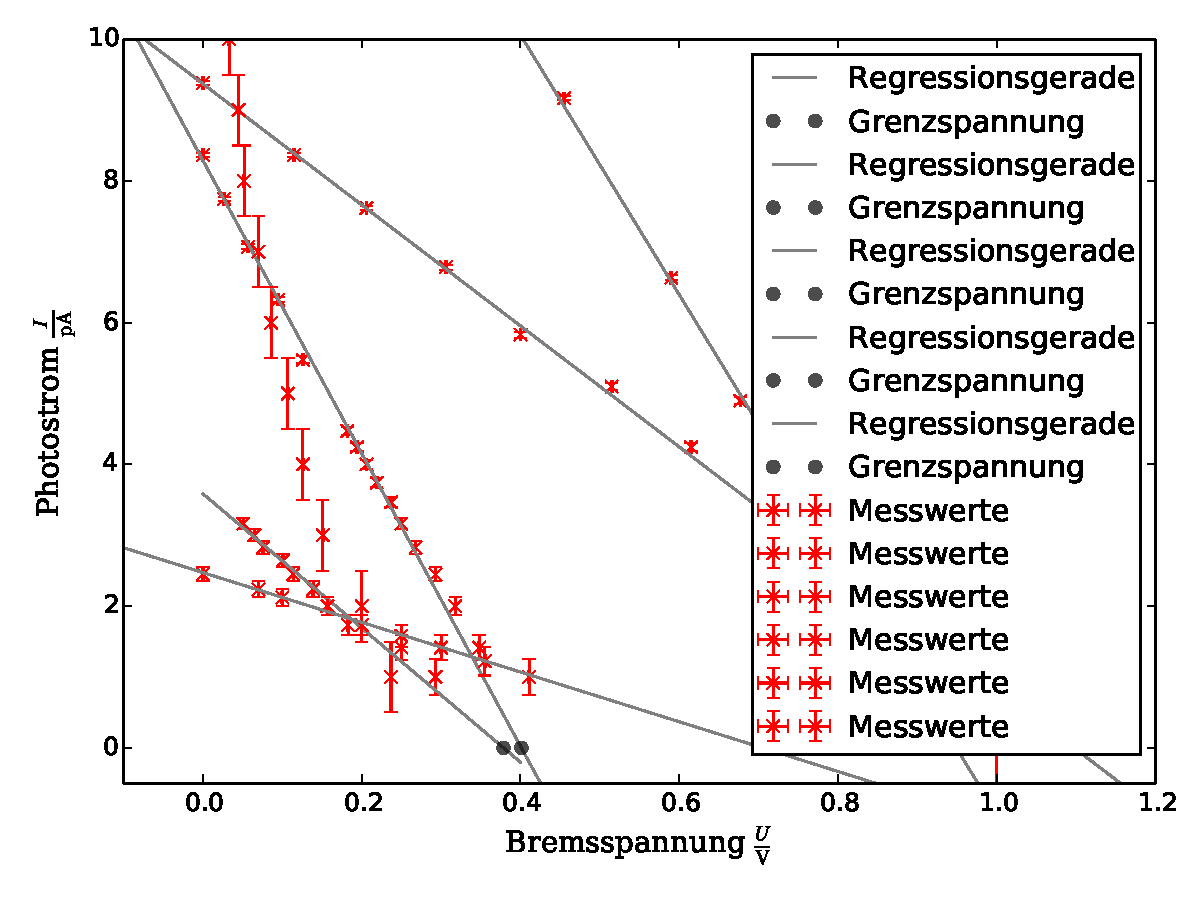
\includegraphics[scale=0.7]{Grafiken/Orange2.pdf}
			\caption{Abhängigkeit des Photostroms von der Bremsspannung \label{fig:Messwerte_Messung2}}
		\end{figure}
		\begin{table}[!h]
	\centering
	\begin{tabular}{|c|c|c|c|}
		\hline
		Photostrom & Bremsspannung & Photostrom & Bremsspannung\\
		$I$ [\si{\pico\ampere}] & $U$ [\si{\volt}] & $I$ [\si{\pico\ampere}] & $U$ [\si{\volt}]\\
\hline\hline
		\num{-2.0(5)} & \num{20.000(1)} & \num{20.0(5)} & \num{-0.052(1)}\\
		\num{-1.0(5)} & \num{16.000(1)} & \num{22.0(5)} & \num{-0.070(1)}\\
		\num{-0.5(5)} & \num{12.000(1)} & \num{24.0(5)} & \num{-0.080(1)}\\
		\num{-0.5(5)} & \num{8.000(1)} & \num{27.0(5)} & \num{-0.095(1)}\\
		\num{-0.5(5)} & \num{4.000(1)} & \num{30.0(5)} & \num{-0.114(1)}\\
		\num{0.0(5)} & \num{1.000(1)} & \num{54.0(5)} & \num{-0.213(1)}\\
		\num{1.0(5)} & \num{0.237(1)} & \num{83.0(5)} & \num{-0.305(1)}\\
		\num{2.0(5)} & \num{0.200(1)} & \num{130.0(5)} & \num{-0.400(1)}\\
		\num{3.0(5)} & \num{0.151(1)} & \num{185.0(5)} & \num{-0.500(1)}\\
		\num{4.0(5)} & \num{0.126(1)} & \num{270.0(5)} & \num{-0.600(1)}\\
		\num{5.0(5)} & \num{0.107(1)} & \num{320.0(5)} & \num{-0.700(1)}\\
		\num{6.0(5)} & \num{0.086(1)} & \num{560.0(5)} & \num{-1.000(1)}\\
		\num{7.0(5)} & \num{0.070(1)} & \num{1500.0(5)} & \num{-2.000(1)}\\
		\num{8.0(5)} & \num{0.052(1)} & \num{2900.0(5)} & \num{-4.000(1)}\\
		\num{9.0(5)} & \num{0.045(1)} & \num{3200.0(5)} & \num{-6.000(1)}\\
		\num{10.0(5)} & \num{0.033(1)} & \num{4000.0(5)} & \num{-10.000(1)}\\
		\num{11.0(5)} & \num{0.020(1)} & \num{4200.0(5)} & \num{-14.000(1)}\\
		\num{12.0(5)} & \num{-0.000(1)} & \num{4400.0(5)} & \num{-16.000(1)}\\
		\num{16.0(5)} & \num{-0.027(1)} & \num{4600.0(5)} & \num{-18.000(1)}\\
		\num{18.0(5)} & \num{-0.039(1)} & \num{4600.0(5)} & \num{-20.000(1)}\\
		\hline
	\end{tabular}
	\caption{Messwerte der orangenen Spektrallinie bei verschiedenen Bremsspannungen \label{tab:Messwerte_Messung2}}
\end{table}


		
	